\documentclass{Resources/UoBLab1}
\pubyear{2019}
\usepackage{listings}
\subjectarea{Microcontroller Lab Report}

\begin{document}
\firstpage{1}

\title{ResQbot}
\vspace{3mm}\vspace{3mm}
\course{Course ID : CSE-3116}
\school{Department of Computer Science and Engineering, University of Dhaka}
\date{Date: 27/04/2019}
\author{Authors/ Project partners
\newline     1. Rafe Samnan------Roll:25\newline     2. Sakib Hasan------Roll:125}
\keywords{Arduino, microcontroller}

\maketitle

\begin{abstract}
The target of this project is to build two robots where one of them will serve as master robot and other would be follower robot that can follow given instructions. The baseline we are aiming for is a “Rescue” task. The leader of them will be instructed to move  from one location to another and give back the path it took via wireless module. Other Robot(s) will follow the leader's path as sent from leader.
\end{abstract}


\section{Introduction}
This robotic system would help in rescue missions as if one robot goes to rescue vivtims and fall under any unexpected circumstances by any means then we have to send back up for maintenance or further initiatives. As the leader robot sends back feedback on every movement on the path it takes and we store it via wireless module system, we can send another probe to that same path to find the victims or leader robot as same way.\newline
This was not a project without hassles and we are expecting quite a few technical difficulties, such as:\newline
Connecting two wifi modules of the two different robots and send data. \newline
Localization the the robots couldn't be handled properly via wifi module, so we had to give manual instruction to master robot.

\section{Theory}
The main idea is to controll one robot(leader) from personal computer via application software to reach victims. The Robot would have a camera onit's main frame to give live feedback on it's path  and we will controll the bot to desired path. The path feedback sent back to terminal will be our log file for leader robot. We can then control the other robot according to the given path as feedabck from leader robot. Hence there will be no need for cameras or other sensors for next batch of robots.\newline
Now to control robot movement we devised an interesting  solution. To minimalize the structural complexity we tried to rotate the bot by changing the movement speed of one wheel respective to other wheel. This technique is sometimes known as "Differential Steering".\newline
This idea helps our robot to take turn without stopping movement at all. \newline
Suppose, velocity of right wheel is \[ v_R\] and speed of left wheel is \[v_L\] , then  to take right turn,  \[v_L >  v_R\] and do reverse for the opposite situtation.


\section{Structure/Design}
\vspace{3mm}
\subsection{Apparatus}
1. Arduino uno/mega 1x for each robot\newline
2. Micro Metal Gear motor 500rpm 2x for each robot\newline
3. NodeMCU 1x per robot\newline
4.Motor driver L298 RED 1 for each robot\newline
5. Metal ballcaster\newline
6. Wheel 2x for each bot\newline
7. Jumper wires\newline
8. Battery\newline
9.Camera/Sonar sensors\newline\newline
Following are the 3D view of the prototype design\newline
\begin{figure}
    \centering
    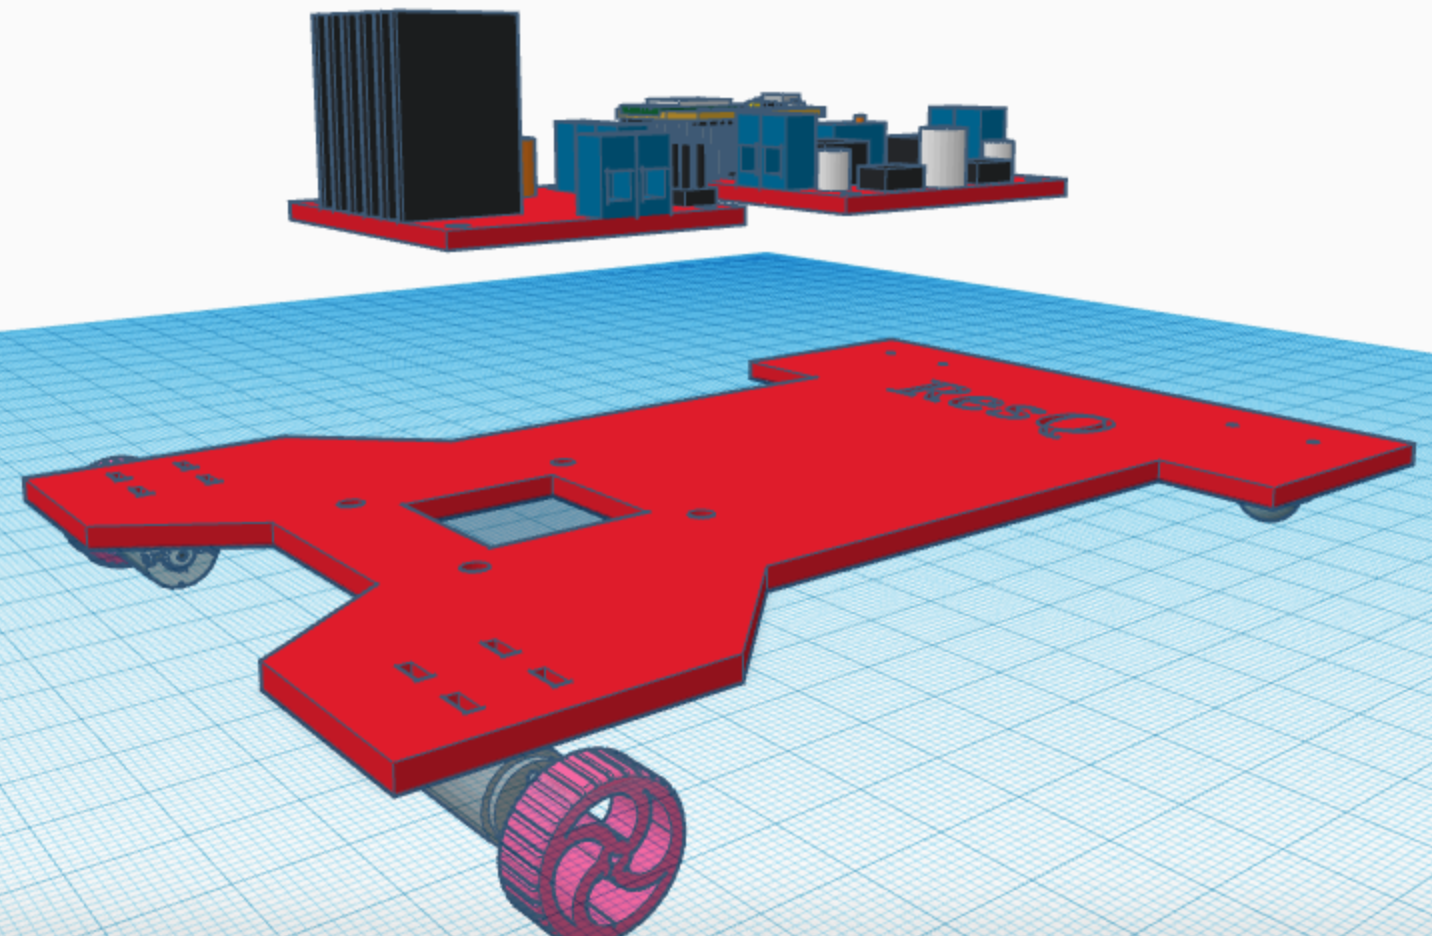
\includegraphics[width=\linewidth]{Resources/comp}
    \caption{Motor driver board and body.\cite{reference1}}
    \label{fig:my_label}
\end{figure}
\begin{figure}
    \centering
    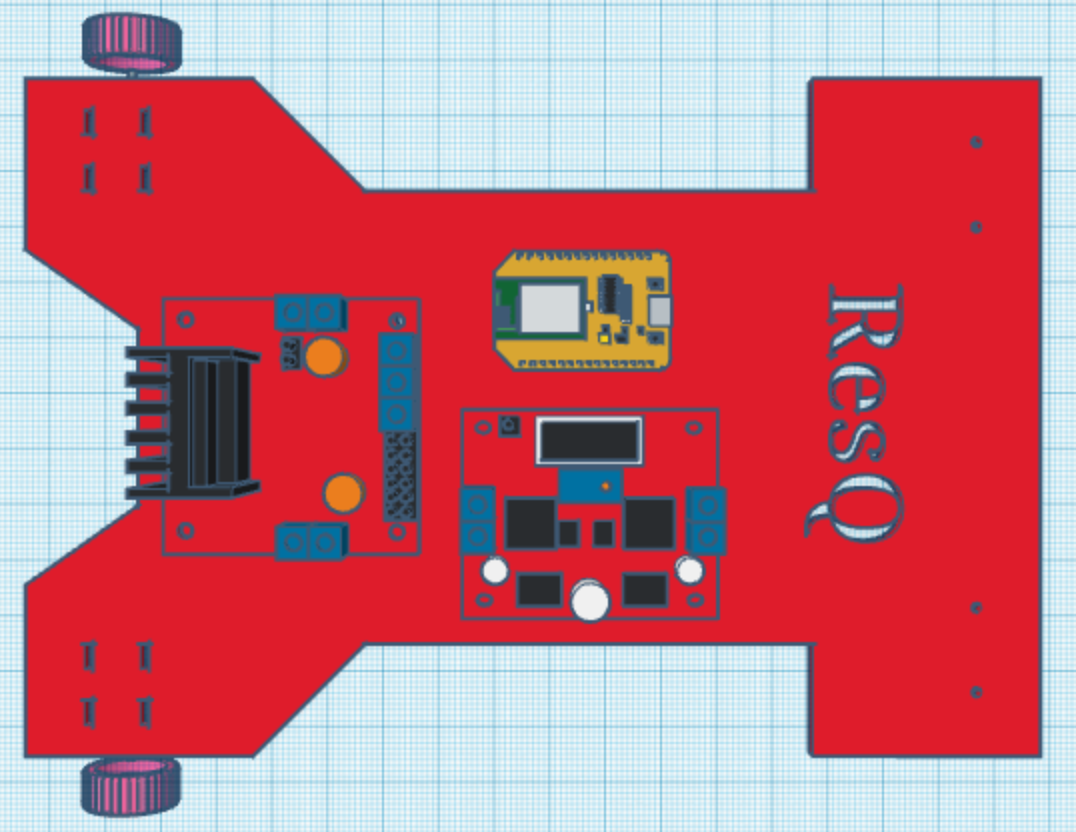
\includegraphics[width=\linewidth]{Resources/top}
    \caption{Top-Corner View.\cite{reference1}}
    \label{fig:my_label}
\end{figure}
\vspace{3mm}
\begin{figure}
    \centering
    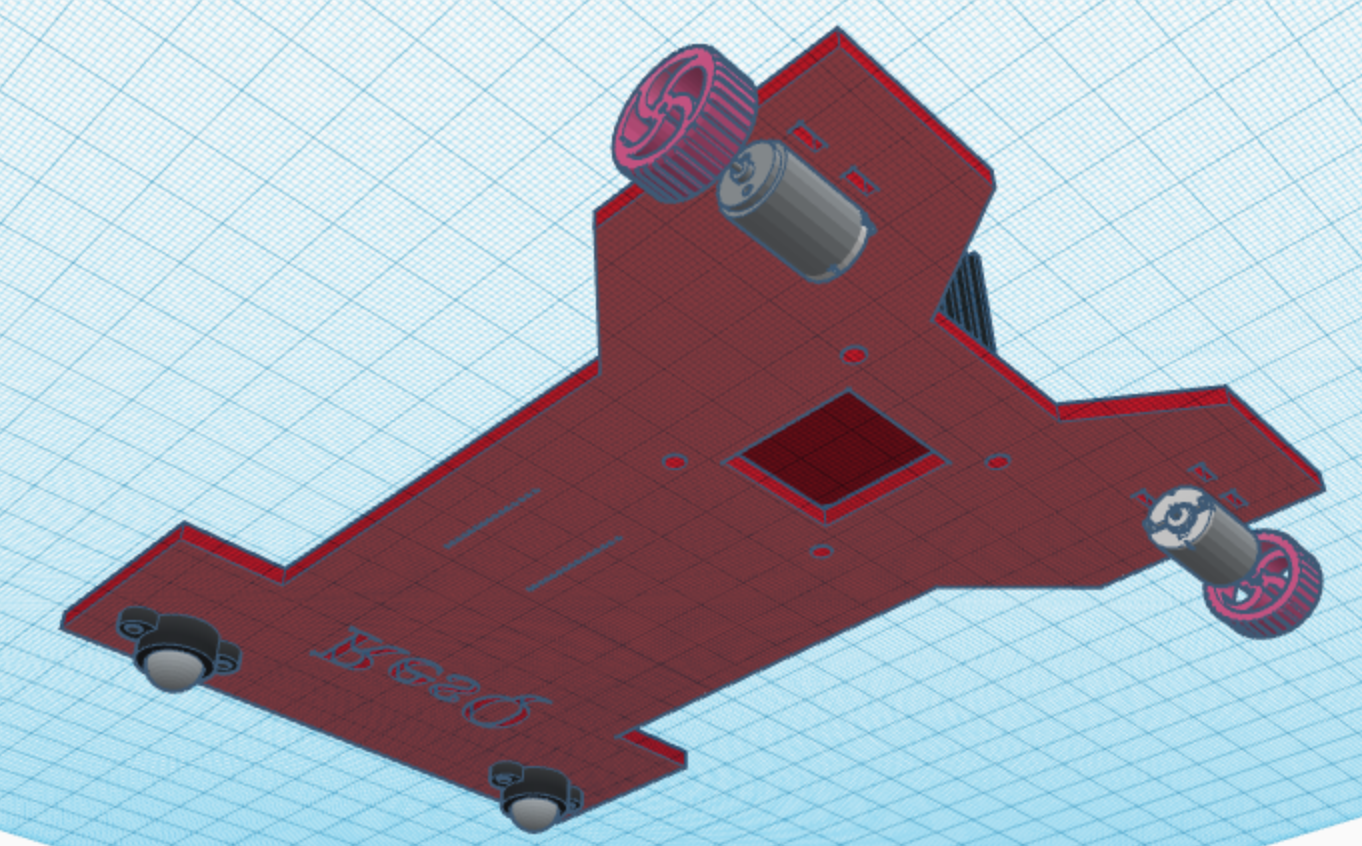
\includegraphics[width=\linewidth]{Resources/bottom}
    \caption{Bottom View.\cite{reference1}}
    \label{fig:my_label}
\end{figure}
\vspace{3mm}
\begin{figure}
    \centering
    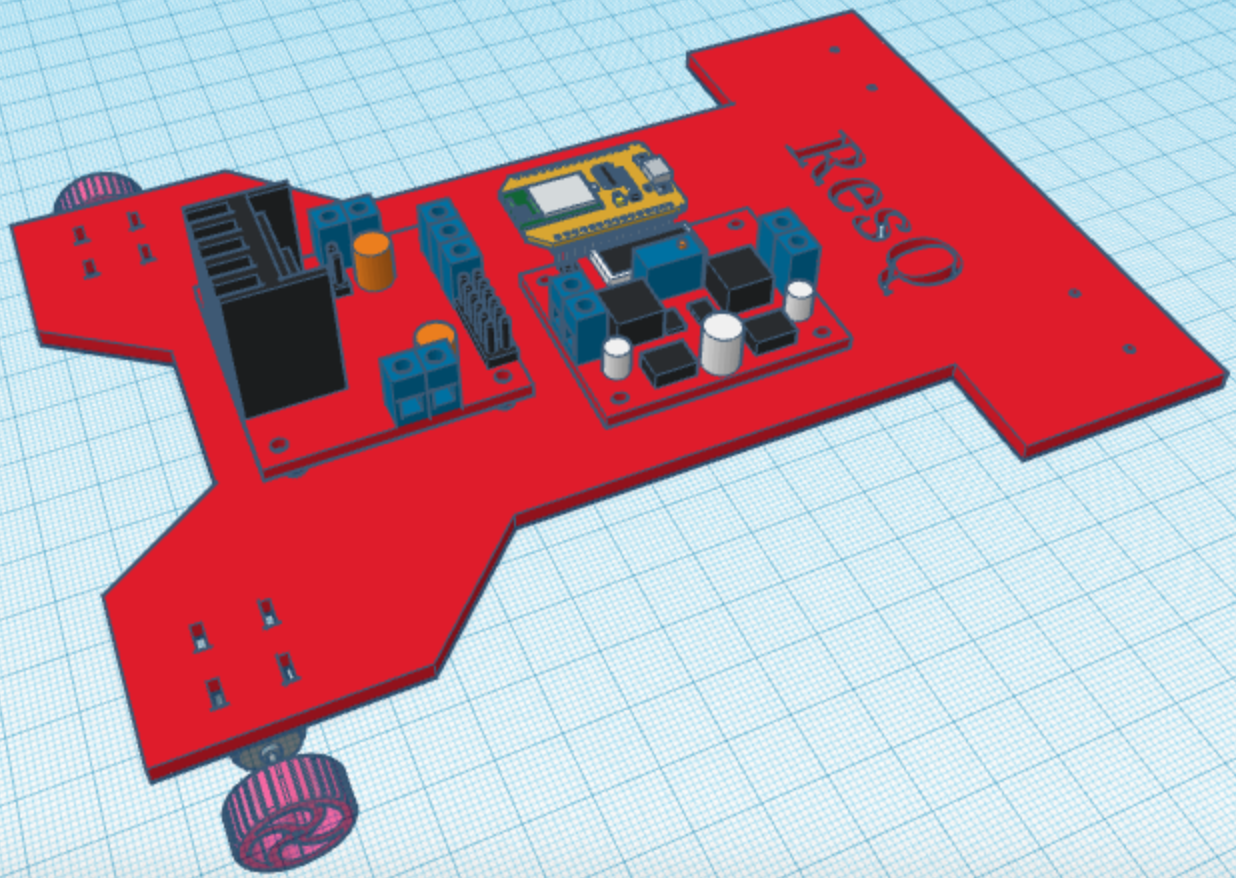
\includegraphics[width=\linewidth]{Resources/corner}
    \caption{Corner side View.\cite{reference1}}
    \label{fig:my_label}
\end{figure}

\subsection{Procedure}

Following are the methods/functions that are used to controll the robots movement and feedback (along with code snippet and explanation).\cite{reference3}-\newline
Function 1-  SetWifi() : works to set up the wifi configuaration for the bot.  it set's up the PC/controlling device as an access point. Then requests for connection and gets input from the controlling devicet or sends back data to output device  via this access point.
\begin{lstlisting}
void SetWifi(char* Name, char* Password)
{
  // Stop Any Previous WIFI
  WiFi.disconnect();

  // Setting The Wifi Mode
  WiFi.mode(WIFI_AP_STA);
  Serial.println("WIFI Mode : AccessPoint Station");

  // Setting The AccessPoint Name & Password
  net_ssid      = Name;
  net_pass  = Password;

  // Starting The Access Point
  WiFi.softAP(net_ssid, net_pass);
  Serial.println("WIFI << " + String(net_ssid) + " >> has Started");

  // Wait For Few Seconds
  delay(2000);

  // Getting Server IP
  IPAddress IP = WiFi.softAPIP();

  // Printing The Server IP Address
  Serial.print("Server IP : ");
  Serial.println(IP);

  // Starting Server
  daServer.begin();
  daServer.setNoDelay(true);
  Serial.println("Server Started, you can connect from the JAVA client");
}
\end{lstlisting}
Function 2 - AvailableClients() : Finds free/disconnected spot , Checks if previously the client is taken or clients connected to the server, disconnect or reject access point.\newline
Function 3 - AvailableMessage() : This function checks clients for data.
\begin{lstlisting}
void AvailableMessage()
{
  //check clients for data
  for (uint8_t i = 0; i < MAXSC; i++)
  {
    if (daClient[i] && daClient[i].connected() && daClient[i].available())
    {
      while (daClient[i].available())
      {
        String Message = daClient[i].readStringUntil('!');
        Serial.println(Message);
        if (Message[0] == 'f') {
          runForward();
        }
        else if (Message[0] == 'r') {
          turnRight();
        }
        else if (Message[0] == 'l') {
          turnLeft();
        }
        else if (Message[0] == 'b') {
          runBackward();
        }
        else if (Message[0] == 'a') {
          stopBot();
        }
        daClient[i].flush();
        for (int i = 0; i < 7; i++)
        {
          int cmd = 97 + i;
          if ((int)Message[0] == cmd)
          {
            digitalWrite(outputIndex[i], HIGH);
            break;
          }
          cmd = 97 + i + 7;
          if ((int)Message[0] == cmd)
          {
            digitalWrite(outputIndex[i], LOW);
            break;
          }
        }
      }
    }
  }
}
\end{lstlisting}
Function 4 - runForward() : To move forward\newline
\begin{lstlisting}
void runForward()
{
  Serial.println("forward");
  analogWrite(leftl, 1023);
  analogWrite(leftr, 0);
  analogWrite(rightl, 1023);
  analogWrite(rightr, 0);
  delay(900);
  analogWrite(leftl, 0);
  analogWrite(leftr, 1023);
  analogWrite(rightl, 0);
  analogWrite(rightr, 1023);
  delay(100);
  analogWrite(leftl, 0);
  analogWrite(leftr, 0);
  analogWrite(rightl, 0);
  analogWrite(rightr, 0);
}
\end{lstlisting}
Function 5 - runBackward() : To go backwards\newline\newline
Function 6 - turnRight() : To turn right\newline\newline
Function 7 - turnLeft()  : To turn left\newline\newline
The implementation idea of fuction 5, 6, 7 are same as function 4.
There is also a java program to create a server connection via custom socket and port for the bot to connect to recieve data or send.

\section{Results}
While moving the leader robot sends feedback on the movement or change back to the controlling device terminal. For example, When moving forward, it prints " Forward" along with speed when turning right prints"Right" and same for backword  movement and left turn. We couldn't use other sensor for shortage of time and scarcity of harware components and time.

\section{Discussion} 
\subsection{Analysis}
We have tested the bots several times to determine which structure would be more stable and less error making. The final prototype has a solid structure and movement can be controlled perfectly 90\% of the time. Connects to access point individually and gets input orders perfectly. Sending feedback from the bots had been a hastle as NodeMCU module or other wifi module doesn'tt support sending customized data or multiple sensor feedback at once. So we had to remove sensors from our structure for now. But this structure could've been improved by using rasberry pi instead of Arduino board. and using camera/sonar along with a display could've make the project more meaningful by presesnting a visualization of real life use.
\subsection{Application Domain}
With the advancement of modern technologies, real life and user end applications of robotics is expanding in an unfathomable pace. There are lots of applications and possibilities for Robotic Swarm technology. Swarm robots have many applications.\newline
* Disaster rescue missions is one of the most important applications of swarms robots. Swarms of robots of could be sent to places rescue workers can't reach this would save lives. \newline
* Swarm robots have many applications that can be used in military to form an autonomous army.  \newline
* Swarm robots are also useful for autonomous surveillance and environment monitoring to investigate environmental parameters, search for survivors, and locate sources of hazards such as chemical or gas spills, toxic pollution, pipe leaks and radioactivity.\newline
* Can also be used in agricultural activities like seeding, watering/nurturing plants and harvesting as well.\newline
* Swarm robots can be used for different physical simulation for algorithms or programs, military or war strategies.\newline
* Swarm robots can be used for navigation. Where the destination can be fixed or derivable and other robots follow the leader or just find and reach individually.

\section{Conclusion}
Finally, we completed the project with minimal complexity and maximum possible feasibility. We didn't have enough time and proper aparatus to try out some other proposed features or test implemented ones. 
We have tested the bots over and over again and the control and feedback of them ar proper in every test cases.The structure is strong enough not to break while moving and connection of wires were properly handled.\newline
But it was a great experience for us to work in this project. We learnt a lot from this project. This learning experience will help in future to work on more projects.This project can be improved and can be made more efficient andusable with proper process and can be used in real life as well.
\section*{Acknowledgements}

We thank Dr. Shugata Ahmed Sir and Dr. MD Mosaddek Khan Sir to instruct us throughout the project. Also, we want to thank all the author of the references we have used throughout our project..\newline
1. Dr. Md. Mosaddek Khan, Dept. of CSE, DU
2. Dr. Shugata Ahmed, Dept. of RME, DU

\begin{thebibliography}{}

\bibitem{reference1}
designed with Autodesk Software
\bibitem{reference2}
https://www.rakeshmondal.info/4-Wheel-Drive-Robot-Design
https://arduino.stackexchange.com/questions/9018/how-to-make-the-motor-car-move-left-forward-left-backward-right-forward-right
\bibitem{reference3}
https://github.com/Geektrovert/NodeMCU-controller/?fbclid=IwAR2RbCWPjFsNA97UvIGOqvguIB8p5RRnWEfCKzfH39ZLN9v2oZvs4ceryaw
\end{thebibliography}

\end{document}
